
Uit de twee simulaties zijn de volgende twee grafieken ontstaan. Figuur \ref{E1} is de grafiek die volgt uit de simulatie met enkele inverter en figuur \ref{E2} is ontstaan uit de simulatie met de drie inverters in cascade.
\\
\\
Uit deze twee figuren kan de vertraging afgeleid worden voor de desbetreffende circuit oftwel de $t_{90\%}$ van het circuit. Uit figuur \ref{E1} kan afgelezen worden dat de vertraging van het circuit met enkele inverter 0,3 s is. 
\begin{figure} [h!]
\centering
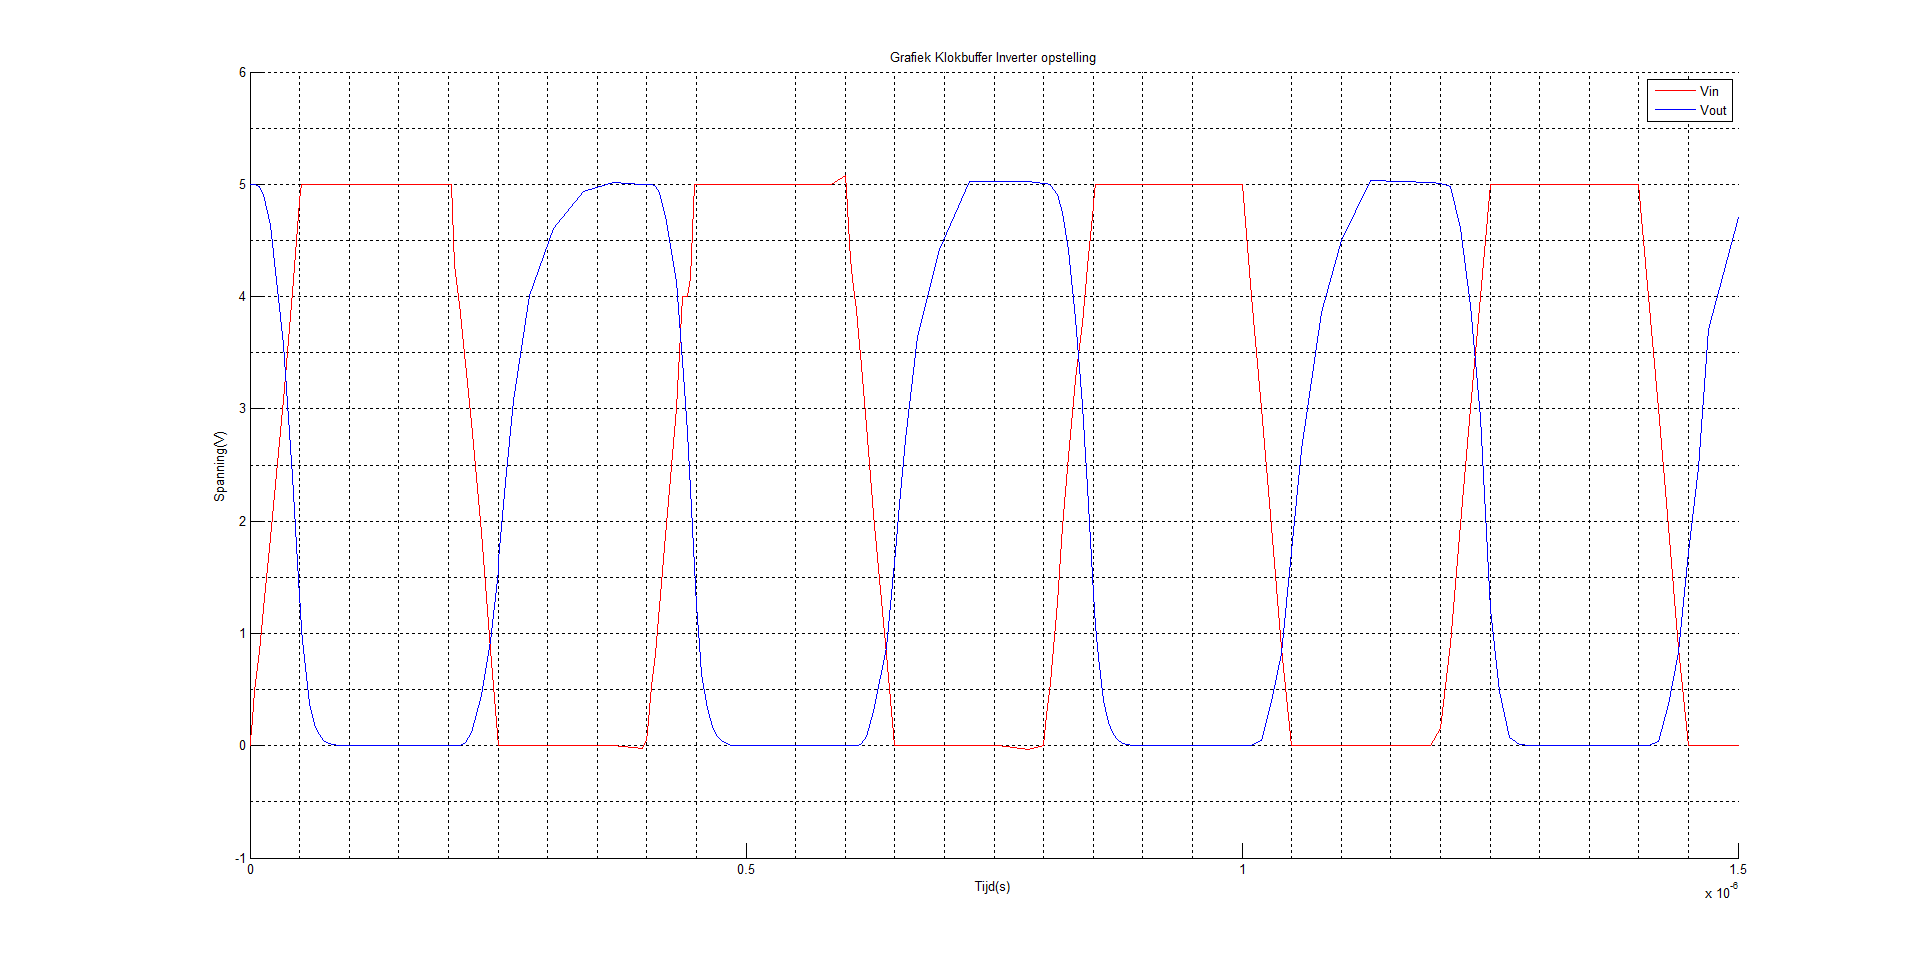
\includegraphics [width = \textwidth] {inputfiles/GrafiekInverter}
\caption{De simulatie resultaten van de enkele inverter in SPICE}
\label{E1}
\end{figure}
\\
Uit figuur \ref{E2} kan afgelezen worden dat de vertraging van het circuit met drie inverters in cascade 0,24 s is.

\begin{figure} [h!]
\centering
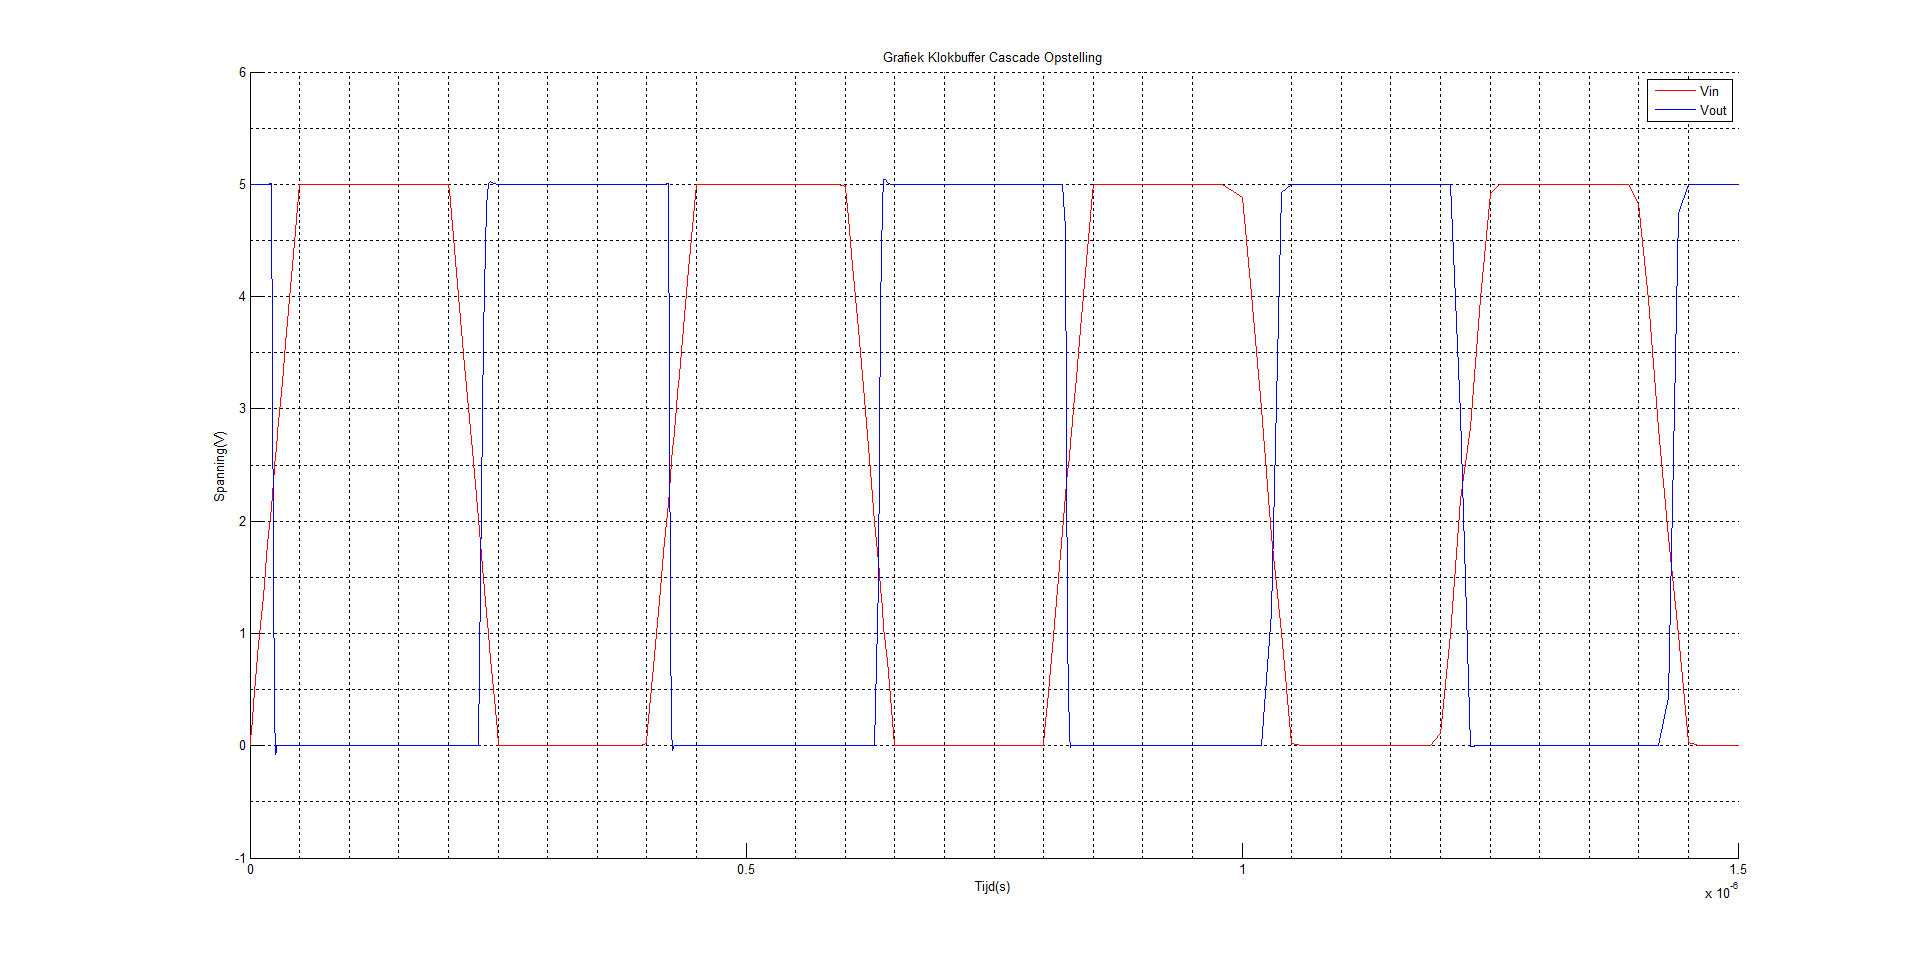
\includegraphics [width = \textwidth] {inputfiles/GrafiekCascade}
\caption{De simulatie resultaten van de driedubbele inverter in SPICE}
\label{E2}
\end{figure}


